\documentclass[12pt,a4paper]{article}

\usepackage[utf8]{inputenc}
\usepackage[T1]{fontenc}
\usepackage{lmodern}
\usepackage[english]{babel}
\usepackage{amsmath}
\usepackage{amsfonts}
\usepackage{amssymb}
\usepackage{graphicx}
\usepackage{tabularx}
\usepackage{url}
\usepackage[a4paper, left=2.5cm, right=2.5cm, top=2.5cm, bottom=2cm]{geometry}
\parskip 12pt
\parindent 0pt


\title{Varying Number of Features of Neural Network Input Objects}
\author{}
\date{}

\begin{document}

\maketitle

\section{Problem}

In a feed forward neural network, each feature of the input objects corresponds to an input neuron of the neural network. But it is unclear what to do if the number of features of the input objects varies.

In the case of particle physics, the input objects can be events in a collider experiment and the purpose of the neural network can be to distinguish between signal and background. Figure~\ref{fig::NN_picture_1} shows a part of such a network. In this example, the fourth input neuron takes $p_\text{T}$ of jet number seven. The question is what to do if there are events with fewer than seven jets.


\begin{figure}
\begin{center}
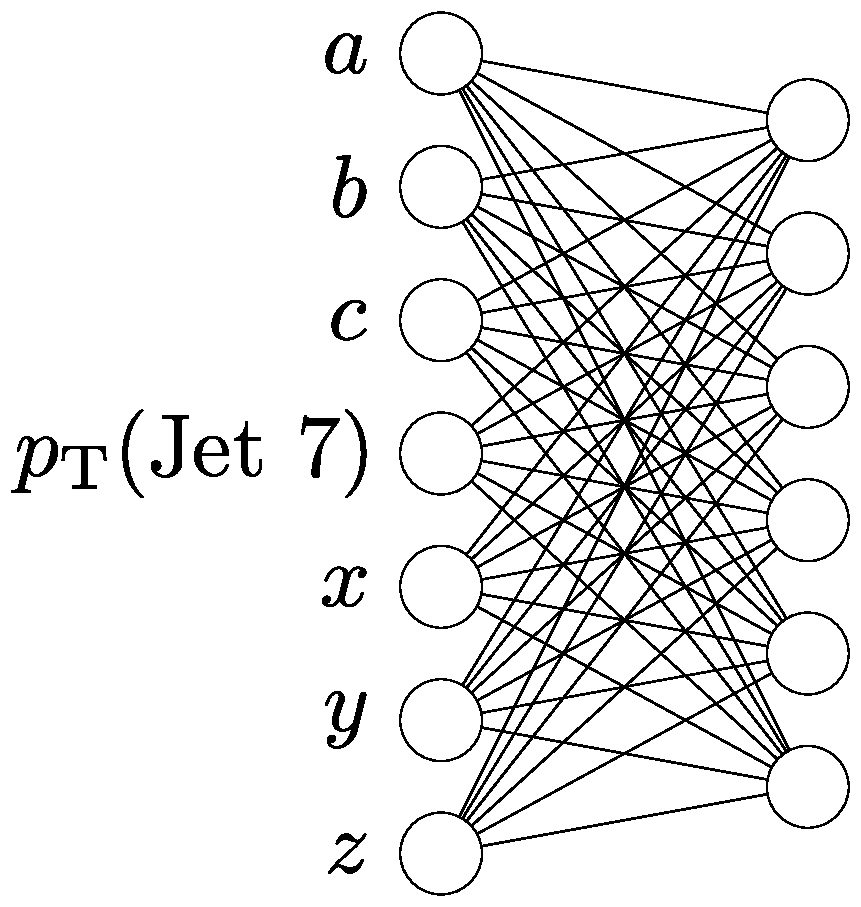
\includegraphics[scale=0.4]{NN_picture_1.pdf}
\caption{Part of a neural network.}
\label{fig::NN_picture_1}
\end{center}
\end{figure}


\section{Possible Solution}
\label{sec::Possible_solution}

\begin{figure}
\begin{center}
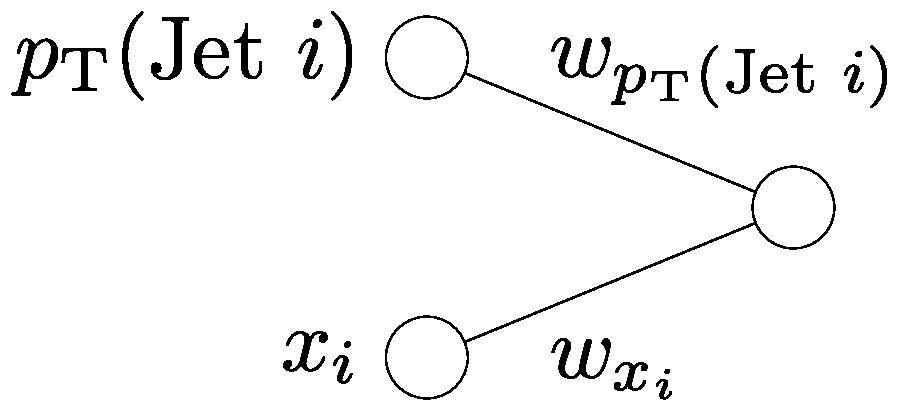
\includegraphics[scale=0.4]{NN_picture_2.pdf}
\caption{Part of a neural network with additional input neuron.}
\label{fig::NN_picture_2}
\end{center}
\end{figure}

A possible solution for this problem is an additional input neuron for each jet. The input of these additional neurons is $x_i = 0$ if the corresponding jet~$i$ exists and $x_i = 1$ if the corresponding jet~$i$ does not exist. If the jet does not exist, the neurons that would take the properties of the jet (e.g.\ $p_\text{T}$) as their input get an arbitrary but fixed value. Equation~\eqref{eq::input_hidden_layer} is a part of the input of the neuron in the first hidden layer (see figure~\ref{fig::NN_picture_2}).
\begin{align}
\dots + p_\text{T}(\text{Jet }i) \cdot w_{p_\text{T}(\text{Jet }i)} + x_i \cdot w_{x_i} + \dotsb \label{eq::input_hidden_layer}
\end{align}

If jet~$i$ exists, the second summand of equation~\eqref{eq::input_hidden_layer} is zero and the input for the hidden neuron is not influenced by the additional input neuron. If jet~$i$ does not exist, the weight $w_{x_i}$ can be used to push the result into the direction of the wanted output for this case.


\section{Results}

The procedure described in section~\ref{sec::Possible_solution} was tested with a network that separates t$\overline{\text{t}}$H(b$\overline{\text{b}}$) signal events from t$\overline{\text{t}}$ + jets (including t$\overline{\text{t}}$b$\overline{\text{b}}$) background events. For comparison, a second network was trained where the jets that do not exist for all events were not used as input at all. The network with the additional jets did not perform better than the other one.


\section{Open Questions}

\begin{itemize}
\item Is there a case where the procedure described in section~\ref{sec::Possible_solution} improves the performance of a neural network?
\item If there is such a case:
\begin{itemize}
\item Is it important, that the additional variable is $x_i = 0$ if the corresponding jet~$i$ exists and $x_i = 1$ if the corresponding jet~$i$ does not exist? Or can you also use the usual system (which is the other way round)?
\item What is the best way to do the feature scaling?
\begin{itemize}
\item Is it a problem if the variables that show whether a jet exists are included in the feature scaling?
\item Should the feature scaling happen before or after the not existing variables are set to a fixed value?
\end{itemize}
\item A possible alternative to the procedure described in section~\ref{sec::Possible_solution} is to introduce more jet btag categories (with 7~jets, 8~jets, \textellipsis\unkern). This is a simpler procedure, but there are fewer training events per category available. Which solution performs better?
\end{itemize}
\end{itemize}


\section{Code Fragment}

The code fragment in the file \url{preprocessing_fragment.py} shows how the procedure described in section~\ref{sec::Possible_solution} can be implemented using the Pandas DataFrame.


\end{document}
